\documentclass{book}

\usepackage[utf8]{inputenc}
\usepackage[T1]{fontenc}
\usepackage[francais]{babel}
\usepackage{graphicx}
\usepackage{adjustbox}
\usepackage{fancyref}
\usepackage{hyperref}
\usepackage{url}
\usepackage[top=3cm, bottom=3cm, left=3cm, right=3cm]{geometry} % pour les marges


\title{%
  Projet de Sciences des Données \\
  \large Explotation d'images satellites haute-résolution \\pour la prévision d'indicateurs socio-économiques \\
    }

\author{\textsc{Youcef} - \textsc{Kacer}}
\date{22 Novembre 2016}

\begin{document}
 
\maketitle

\tableofcontents

\frontmatter
\chapter{Introduction}
Dans ce document, nous présentons les premiers de résulats de classiifcation des communes françaises, à partir de leur histogramme de $NDVI$. Nous cherchons ainsi à pédire
la densité de population de chaque commune. 

\mainmatter
\chapter{Données Landsat-8 pour la France métropolitaine}

Nous avons récupéré des scènes Landsat-8 couvrant la France métropolitaine entre le 15 Mai 2015 et le 15 Septembre 2015.\\
Cette période est la plus courte permettant d'avoir une converture totale du territoire métroplitain tout en conservant une couverture nuageuse inférieure à 10\%.
Nous obtenons ainsi 70 scènes Landsat-8 chacune correspondant à un couple $path$,$row$ unique.\\
Les figures \ref{cloud1},\ref{cloud2} et \ref{cloud3} montrent des miniatures couleurs des 3 scènes ayant la plus forte couverture nuageuse

la figure \ref{couverture} présente toutes les scènes après projection en Web Mercator (EPSG:3857) (repère absolu).

\begin{figure}
\begin{center}
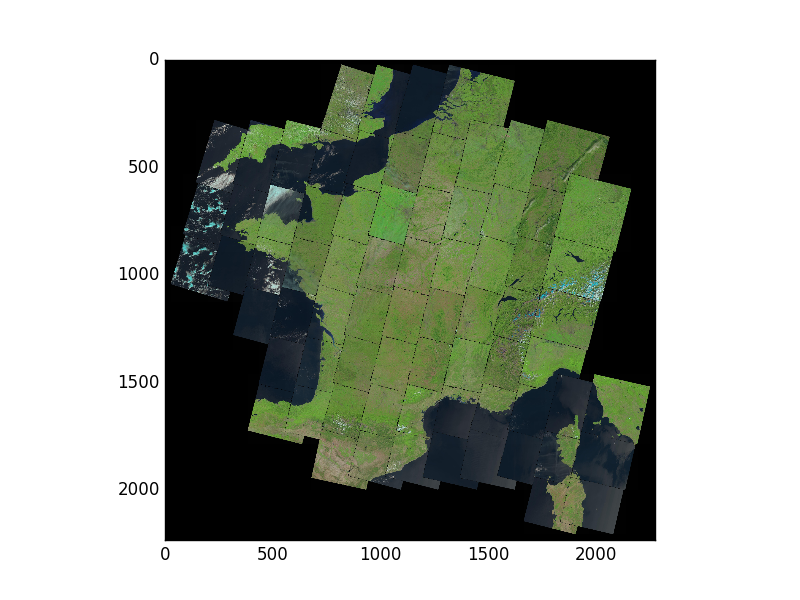
\includegraphics[scale=0.6]{images/france-covering.png}
\end{center}
\caption{Concaténation des 70 scènes Lansat-8 après projection en Web Mercator (EPSG:3857)}
\label{couverture}
\end{figure}
\clearpage

\chapter{Extraction de l'histogramme de NDVI}

Nus avons à disposition un fichier de 36700 comunes françaises contenant entre autre, la latitude et la longitude, la surface, la densité de population en 2012 ainsi
que la population en 2010.\\
Afin d'obtenir des longitudes, latitude précises, nous les avons corrigés en utilisant une API Python de géolocalisation $geopy$ \cite{geopy}.\\
on projète les latitude et longitude en Web Mercator pour chacune des communes. Les positions $x$,$y$ obtenues permettent d'aller récupérer la scéne Landsat-8
L'INSEE définit quatre types de communes en fonction de la densité de population. Nous reprenons ci-après la nomenclature telle que définie sur le
site de l'organisme public \cite{insee}:\\

\begin{quotation}
\begin{itshape}
La nouvelle typologie de l’Insee s’inspire de la classification européenne urbain-rural conçue à partir des données carroyées de population. 
Elle permet de définir 3 types d’espace :\\

\begin{description}
\item[les communes densément peuplées :] dont la densité de population au carreau est d’au moins 1 500 habitants par km\textsuperscript{2} 
et qui comptabilisent un minimum de 50 000 habitants ;

\item[Les communes de densité intermédiaire :] les carreaux contigus ayant une densité de population d’au moins 300 habitants par km\textsuperscript{2} 
et un minimum de 5 000 habitants ;

\item[Les communes peu denses :] les carreaux contigus ayant une densité de population de moins de 300 habitants par km\textsuperscript{2} 
et moins de 5 000 habitants.
Avec cette typologie, 90 \% des communes françaises sont « rurales ». L’Insee rajoute alors un 4e degré en partant de la «maille rurale » (peu dense) :

\item[les communes très peu denses :] carreaux de densité de population d’au moins 25 habitants par km\textsuperscript{2} et moins de 300 habitants
\end{description}
\end{itshape}
\end{quotation}


\clearpage
%Paris 21288
%Versailles 3289
%Fontainebleau 89
%Melun 4924
%Albertville 1076
%Annecy 3690
%Chambéry 2731
%Chamonix-Mont-Blanc 76
%Bourg-en-Bresse 1680
%Lyon 10117
%Thonon-les-Bains 2092
%Montpellier 4524
\backmatter

\listoftables

\listoffigures

\bibliographystyle{alpha}
\bibliography{biblio}

\end{document}